\chapter*{General introduction }

The agriculture industry is faced with greater demands of increased productivity with limited environmental impact and minimal safety risk to the workers. While a wide array of issues needs addressing in this sector, pesticide application remains an essential yet unsafe practice. Current pesticide application involves spraying which not only exposes farmers to hazardous chemicals but is inefficient in pesticide utilization and harmful for the environment due to excessive or uneven pesticide application. As the demand for food continues to rise, innovative and safe as well as economical farming practices are ever-increasingly being sought.

In this context, robotics and automation present a very attractive solution to bring modernization into agricultural activities. Automation by implementing robot systems in the field can perform some tasks which require precision, control or a robot action, are either laborious, highly repetitive or dangerous for humans. The scope of this project is to design and develop a robotic system for pesticide spraying. The robot intends to optimize pesticide application process by the introduction of improved accuracy, limited exposure to humans and limited amount of pesticides use. Integrated with mechanical design, embedded system and smart control, the system is proposed to help sustainable farming as part of an overall trend toward precise agriculture.

The project includes conceptual design, hardware implementation, software design of a spraying robot. The work is also evaluating the system performance: efficiency, reliability, applicability in several farming contexts. Overall, the objective of this work is demonstrating how robotics solutions can assist solving practical issues in agriculture and enabling more sustainable and productive farming.

\chapter{State of the art in Agricultural Robotics and AI}

\section{Introduction}
\subsection{Agricultural Automation and Technological Evolution}


In modern, increasingly complex agriculture, the uptake of advanced technology for improved efficiency, productivity and sustainability is expanding. Traditional farming approaches that heavily rely on manual labor and uniformity in input application are now being substituted by a more data driven and automated system, due to the requirement of optimising resource use, reducing cost of operation and adhering to environmental pressures. Data collection tools like sensors, IoT devices and data analytics are now extensively applied in agricultural processes, leading to efficient and effective decision-making based on the real time data collected \cite{Wolfert2017}.

Precision agriculture has been a significant concept in this transformation process. It revolves around performing the right application, at the right spot, at the right time, reducing waste and optimizing operations. Through the integration of spatial data, environmental sensing technologies and computing tools, farmers are able to shift from reactive management to proactive agricultural system. This shift not only leads to a higher yield but also minimize the negative impact on environment.

% Suggested figure:
 \begin{figure}[H]
 \centering
 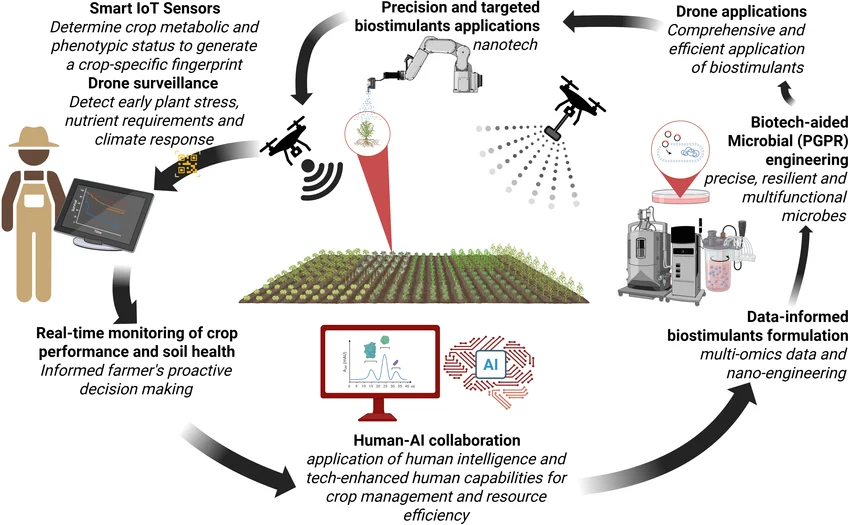
\includegraphics[width=0.6\linewidth]{figures/precision_agriculture.png}
 \caption{Conceptual illustration of precision agriculture with integrated sensors and data-driven decision-making.}
 \label{fig:precision_agriculture}
 \end{figure}
% Use this if you want to visually introduce the idea of smart farming ecosystems.


\subsection{Emergence of Agricultural Robotics and Artificial Intelligence}

In the sense of precision agriculture, robots and Artificial Intelligence (AI) were being utilized in highly specific and tedious agricultural tasks. The agricultural robot is often called agribot, as its duty is to achieve high accuracy and uniformity in agriculture operations in changing environmental conditions of the field. They are the product of the multidisciplinary combination of mechanical structure, embedded electronics and intelligent algorithms for their operation in complicated agriculture systems \cite{Bechar2016}.

The primary features of the agricultural robotics systems can be categorized into:

\begin{itemize}

\item \textbf{Automation of field operations:}  
Agricultural robots can accomplish numerous tasks such as sowing, harvesting, spraying, and crops monitoring. These tasks are achieved with great repeatability and less human workforce involved, thus enhancing operational efficiency.

\item \textbf{Integration of intelligent perception systems:}  
Through computer vision, robots use cameras and sensors to sense their surroundings. The vision system helps robots identify crops, weeds and pests in real time that is used to make robotic decisions.

\item \textbf{Use of machine learning and deep learning:}  
These recent breakthroughs in deep learning have dramatically improved the effectiveness of detection and classification methods, enabling real-time, high-precision object identification, and consequently providing potential applications in the context of precision agriculture \cite{Kamilaris2018}.

\item \textbf{Precision and targeted intervention:}  
It allows the robot to carry out selective activities with perception and actuation. An example is the selective spraying of pesticides, which minimize chemicals used, its negative impact on the environment and enhance treatment effectiveness.

\item \textbf{Adaptability to dynamic environments:}  
Agricultural environments are by nature unpredictable and diverse. A robotic system needs to be robust and adaptable to dynamic conditions such as changing ground topography, lighting, and crop distribution.

\end{itemize}


% Suggested figure:
 \begin{figure}[h]
 \centering
 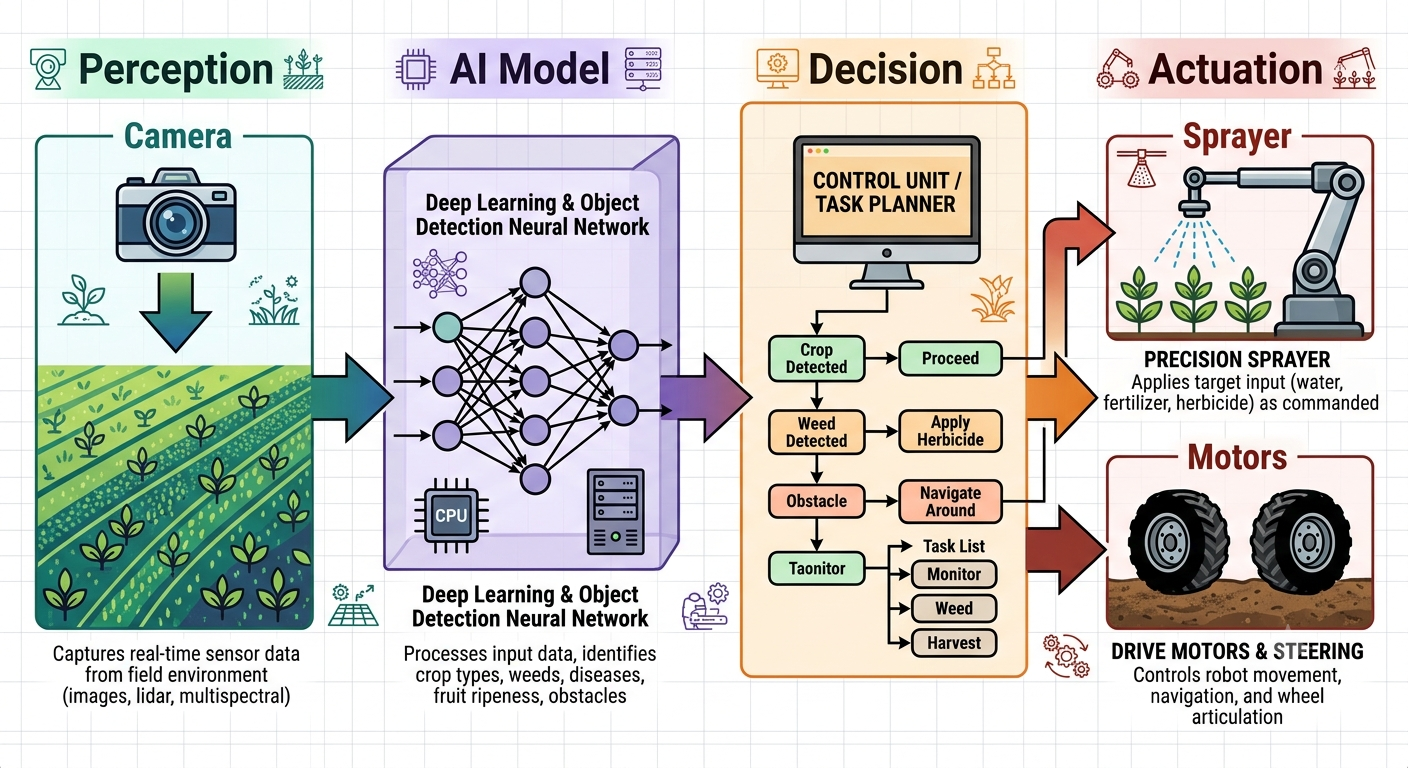
\includegraphics[width=0.8\linewidth]{figures/agri_robot_pipeline.png}
 \caption{Core pipeline of an agricultural robotic system: perception, decision-making, and actuation.}
 \label{fig:agri_pipeline}
 \end{figure}
% This figure works very well here. Keep it simple: Camera → AI Model → Decision → Sprayer/Motors.

\subsection{Overview of Agricultural Robotics}
\subsubsection{Definition and Scope of Agricultural Robotics}

Agricultural robotics refers to design, development and implementation of robotic systems capable of partially or fully automating the accomplishment of agricultural operations. These robotic systems can typically possess perception, sensing, decision making, actuation etc capabilities enabling them to operate in the un-structured and dynamic environments of fields \cite{Santos2021}. While traditional mechanization mainly deals in delivering mechanical power, robotics deal in enabling autonomous, adaptive and intelligent behavior.

Precision agriculture paradigm is tightly connected with the Agricultural robotics. The goal of precision agriculture is to precisely control and spatially and temporally distribute water, fertilizer, and pesticides. The robots, on the other hand, offer a way to achieve such precise and repeatable operations at the field level \cite{Liakos2018}, by functioning as the physical agent that applies the smart decision derived from data at the field level.


% Suggested figure:
 \begin{figure}[H]
 \centering
 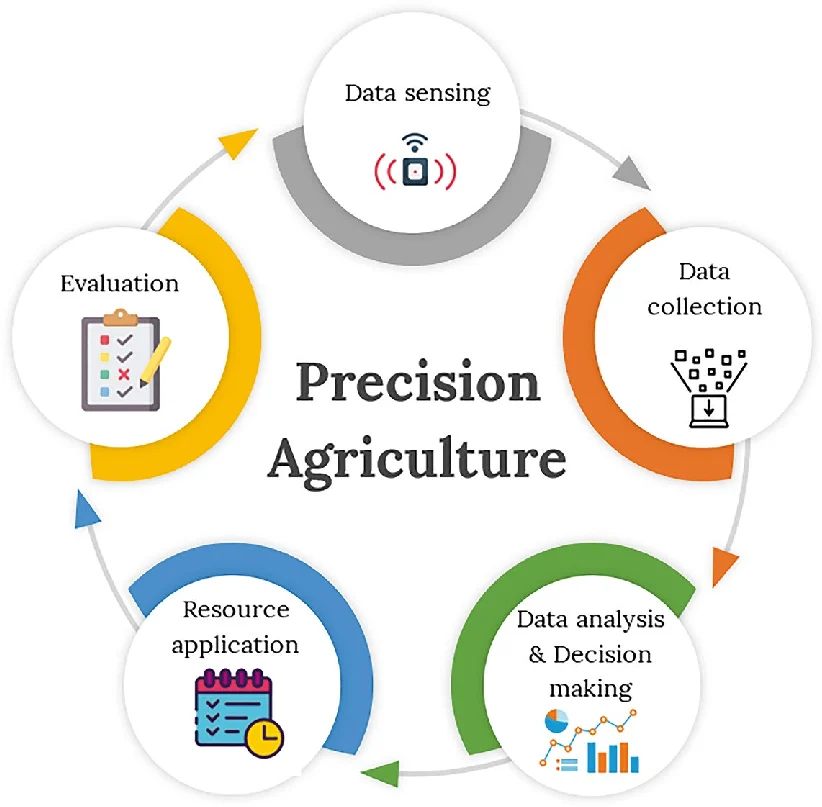
\includegraphics[width=0.6\linewidth]{figures/agri_robot_concept.png}
 \caption{Conceptual relationship between precision agriculture, sensing, data analysis, and agricultural robotics.}
 \label{fig:agri_robot_concept}
 \end{figure}
 %Use this to visually show: Sensors $\rightarrow$ Data/AI $\rightarrow$ Robot actions in the field.


\subsubsection{Evolution of Agricultural Robots}


The development path of agricultural robots can be seen as one progressing from conventional mechanical operation to modern unmanned automated operation. Early forms of agricultural machinery, including tractors and harvesters, essentially replaced labor, providing merely mechanical operation and requiring the input of an operator. Productivity was enhanced but systems were almost devoid of autonomous operation; their functionality was directly dependent on the user's skill.

The second generation of automated machines includes semi-autonomous machines like GPS-controlled tractors, as well as implements that assist in steering and are able to spray at variable rates. These machines employed relatively simple sensors and control logic to enhance the precision of the machine while diminishing the operator's burden \cite{Pedersen2006}. Recently, due to increased development in robotics, computer science and artificial intelligence, totally autonomous robots that perform the tasks of harvesting, spraying or weeding were created. Usually, these robots perform specialized tasks as a series of individual, small robots rather than large multi-purpose machines \cite{Karkee2021}.


\begin{table}[H]
    \centering
    \caption{Evolution of agricultural machinery toward autonomous robots}
    \label{tab:evolution_robots}
    \small % Ensures a clean font scaling for the table data
    \setlength{\extrarowheight}{4pt} % Adds slight padding inside cells for better readability
    
    % \textwidth forces the table to fit the page exactly.
    % 'l' leaves the first column at natural width.
    % 'X' tells the remaining two columns to wrap text and share space equally.
    \begin{tabularx}{\textwidth}{l X X}
        \toprule
        \rowcolor[HTML]{2C3E50} % Elegant dark header row
        \textcolor{white}{\textbf{Stage}} & 
        \textcolor{white}{\textbf{Characteristics}} & 
        \textcolor{white}{\textbf{Human Involvement}} \\
        \midrule
        
        Traditional mechanization & 
        Tractors, harvesters, fixed-rate spraying & 
        Full manual control \\
        
        \rowcolor[HTML]{F2F4F4} % Soft background stripe for readability
        Semi-autonomous systems & 
        GPS-guided tractors, assisted steering & 
        Supervised operation \\
        
        Autonomous robotic platforms & 
        Task-specific robots for harvesting, weeding, spraying & 
        Minimal supervision \\
        \bottomrule
    \end{tabularx}
\end{table}

\subsubsection{Current Applications and Benefits of Agricultural Robotics}

Agriculture robotics is now deployed in a variety of field and greenhouse environments. Some examples of typical usage are:


\begin{itemize}
    \item \textbf{Crop monitoring:}  
   Cameras and sensors on robots and UGVs can gather highly detailed information on the health, development and stress in plants, detecting disease and abnormality early on \cite{Duckett2018}.

    \begin{figure}[H]
    \centering
    % Adjust width (e.g., 0.8 or 0.85) based on your image aspect ratio
    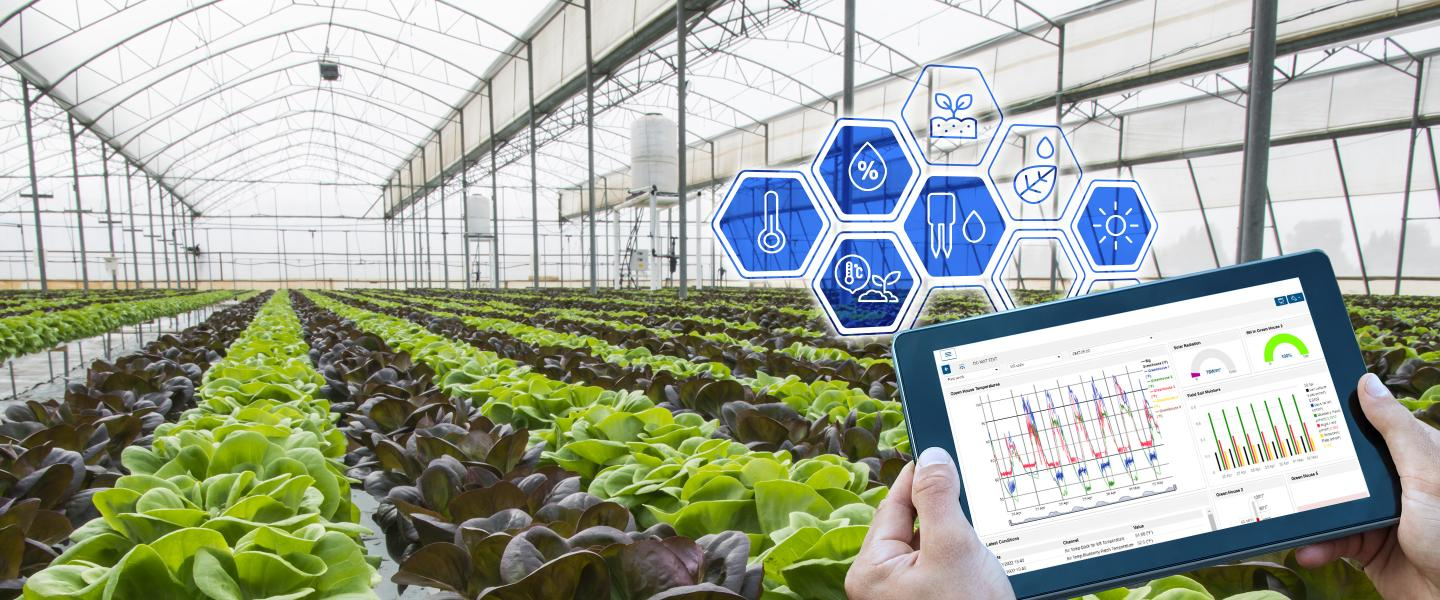
\includegraphics[width=0.85\textwidth]{figures/Crop monitoring.jpg} 
    \caption{Overview of an automated crop monitoring workflow, showcasing real-time data collection via drone/camera payloads and subsequent vision processing.}
    \label{fig:crop_monitoring_workflow}
    \end{figure}
    

    
    \item \textbf{Harvesting:}  
    Robotic harvesting mechanisms aim to achieve produce damage reduction, ease a shortage of agricultural workers, and a degree of scheduling flexibility \cite{Bac2014}.


    \begin{figure}[H]
    \centering
    % Adjust width (0.8 or 0.85) based on your image size
    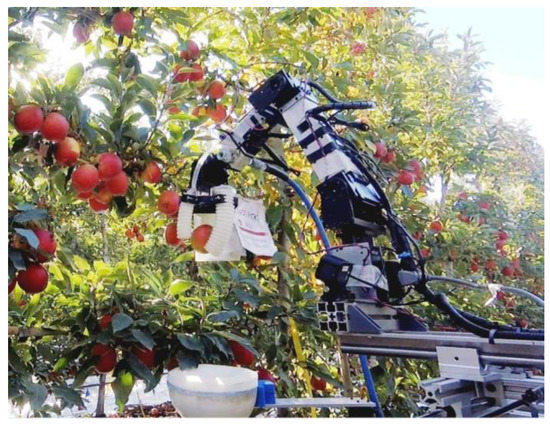
\includegraphics[width=0.6\textwidth]{figures/Harvesting.jpg} 
    \caption{Robotic harvesting architecture, highlighting the integration of a robotic manipulator, end-effector control, and vision-based crop localization.}
    \label{fig:harvesting_system}
    \end{figure}

    
    \item \textbf{Precision spraying:}  
    By installing sprayers in mobile robots, it is possible to precisely apply pesticides or fertilizers to crops. With such machines, chemical amounts and application uniformity can be significantly improved over traditional methods\cite{Sujatha2022}.

    \begin{figure}[H]
    \centering
    % Adjust width (0.8 or 0.85) based on your image size
    \includegraphics[width=0.6\textwidth]{figures/Precision spraying.jpg} 
    \caption{Architecture of a precision spraying loop, mapping target localization data to real-time micro-dose nozzle actuation.}
    \label{fig:precision_spraying_system}
    \end{figure}
    
    \item \textbf{Weed detection and control:}  
    Vision-guided robots are able to differentiate crops and weeds and provide site-specific weed control through physical means (weeding) or application of chemicals (spot spraying).

    \begin{figure}[H]
    \centering
    % Adjusted to 0.75\textwidth to keep it slightly more compact and clean
    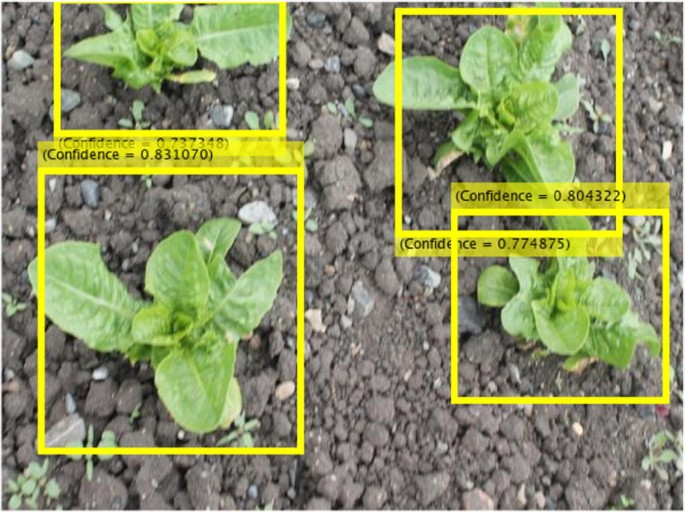
\includegraphics[width=0.6\textwidth]{figures/Weed detection and control.jpg} 
    \caption{Weed detection and spatial control processing loop, showcasing image input segmentation, localized boundary box generation, and precision targeting coordinates.}
    \label{fig:weed_detection_system}
    \end{figure}
    
    \item \textbf{Field inspection and data collection:}  
    Robots assist in day-to-day inspection work, map field conditions and collect information for input into farm management and decision support systems.
\end{itemize}


\begin{figure}[H]
    \centering
    % Scaled to 0.75\textwidth to look uniform with your previous figures
    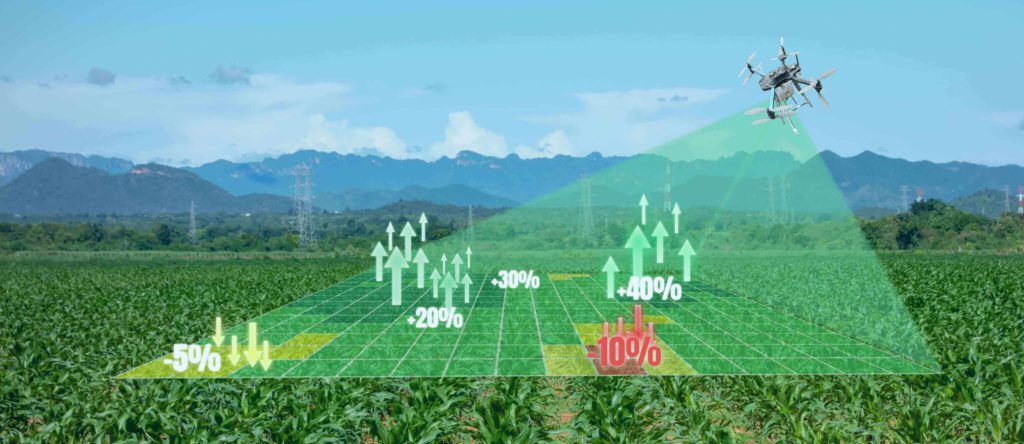
\includegraphics[width=0.75\textwidth]{figures/Field inspection and data collection.jpeg} 
    \caption{Data flow architecture for localized field inspection, mapping physical sensor inputs on the mobile platform to cloud database storage.}
    \label{fig:field_inspection_data}
\end{figure}



    

In terms of benefits there are four major factors that are leading to the adoption of agricultural robotics:

\begin{itemize}
    \item \textbf{Reduced labor requirements:}  
    They compensate for a labor shortage and reduce reliance on manual, seasonal labor in repetitive, potentially dangerous tasks. \cite{Roldan2021}.
    
    \item \textbf{Increased efficiency and productivity:}  
    The high precision and stability of operation facilitate efficient use of inputs and assured task completion over long hours.
    
    \item \textbf{Improved crop management:}  
    Collecting rich data more often allows for better decisions to be made, enabling growers to make interventions quickly, leading to improved crop health and yield. 
    
    \item \textbf{Reduced operational costs:}  
    Increased use of inputs and decreased use of labor costs might eventually lead to the decrease of the cost of production with the increase in time and for scale or labor intensive production processes.
\end{itemize}

Physical task automation by robots is promising but performance of robot in the field is critically dependent upon its intelligence. In order to function efficiently and safely in the unstructured and semi-structured agricultural fields, the robots must be able to infer information from the sensor readings, have better understanding of its environment and appropriately alter its behavior. Therefore it has motivated the implementation of computer vision and artificial intelligence technologies for the robotic platforms for agriculture.


% Suggested figure:
 \begin{figure}[h]
 \centering
 
\includegraphics[width=0.85\linewidth]{agri_robot_applications.png}
 \caption{Examples of agricultural robot applications: monitoring, harvesting, spraying, and weeding.}
 \label{fig:agri_robot_apps}
 \end{figure}
% Only add this if you have clear images or icons; otherwise, keep it textual to avoid clutter.










\subsection{Toward Intelligent Agricultural Robotic Systems}

Automation, robotics, and artificial intelligence came together for creation of intelligent robotic systems in agriculture. The robots have been designed for executing planned tasks or making decisions based on real time data. Perception, processing and actuation together give a robot a ability to act based on circumstances.

Productivity increase at the same time reduce consumption of resources and influence on the environment is the main goal of the development of smart agricultural robots. Specifically for the application of pesticides, smart robots need to achieve detection of diseased parts and application of pesticides only to these parts, so it is possible to avoid unnecessary pesticides and achieve sustainable agriculture \cite{Zhang2018}.

With continued advancement in agricultural systems, intelligent robotics is anticipated to gain greater importance, presenting the scalable, adaptable solutions to some of the major problems of agriculture in this age.

\begin{figure}[H]
    \centering
    % Adjust the width (0.8) to make the image fit nicely on your page
    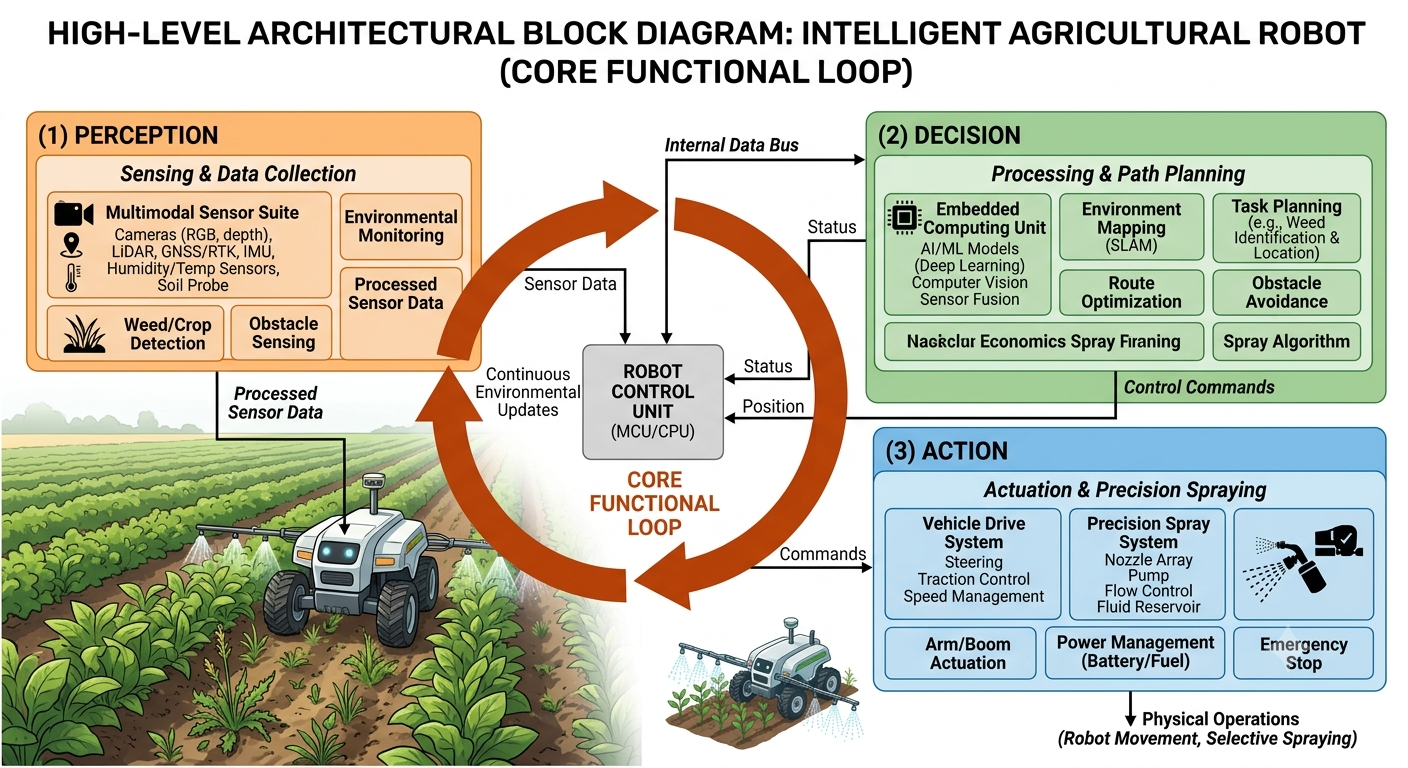
\includegraphics[width=0.8\textwidth]{figures/robot_block_diagram.png} 
    \caption{High-level architectural block diagram of an intelligent agricultural robot illustrating the core functional loop: Perception (sensing and data collection), Decision (processing and path planning), and Action (actuation and precision spraying).}
    \label{fig:robot_high_level_architecture}
\end{figure}



\section{Artificial Intelligence in Agriculture}

\subsection{Artificial Intelligence in Modern Agriculture}

Computation techniques to allow machines to undertake tasks usually performed by humans (e.g. Perception, learning, reasoning, decision making etc.) are broadly known as Artificial Intelligence (AI) \cite{UnderstandingAI2022}. When used in agriculture, these systems allow the large and diverse volume of information from sensors, satellites, agricultural machinery and past records to be processed in order to facilitate more accurate, better informed, more timely decisions through all phases of the agricultural production cycle \cite{AIReview2025}. When coupled with connectivity and automation, this shift the paradigm from experiential farming to predictive and data-driven management.

AI has been and will be a key component in precision agriculture, enabling actionable information to be derived from data and linked to spatially and temporally defined interventions. Use of machine learning and deep learning algorithms to predict these complex interactions between environment, crop condition, and management strategies provides mechanisms to optimize inputs, manage risk, and consequently increase resource-use efficiency, reduce production uncertainty, and increase system robustness \cite{AppsAgri2022}.

\begin{table}[H]
\centering
\caption{Roles of AI in precision agriculture}
\label{tab:ai_roles_precision}
\small
\setlength{\extrarowheight}{5pt} % Adds professional vertical padding inside cells

% \textwidth forces the table to lock onto your document margins.
% 'l' keeps the role names neat; 'X' allows the descriptions to wrap perfectly.
\begin{tabularx}{\textwidth}{l X}
\toprule
\rowcolor[HTML]{2C3E50} % Matching dark slate header block
\textcolor{white}{\textbf{Role}} & \textcolor{white}{\textbf{Description}} \\
\midrule

Data integration & Fusion of sensor, satellite, and historical data for analysis \\

\rowcolor[HTML]{F2F4F4} % Light gray stripe
Decision support & Recommending actions for irrigation, fertilization, and treatment \\

Prediction       & Yield forecasting, disease risk estimation, weather impact modeling \\

\rowcolor[HTML]{F2F4F4} % Light gray stripe
Automation       & Enabling autonomous or semi-autonomous machine operation \\
\bottomrule
\end{tabularx}
\end{table}

%%%%%%%
\subsection{Major Applications of AI in Agriculture}

AI technologies are being used across the different stages of the production cycle and to tackle various agricultural issues. Main application areas are:

\begin{itemize}
    \item \textbf{Crop disease detection:}  
    By employing CNN and other deep learning models, disease symptoms are detected from leaf images and canopy images. It achieved good accuracy of classification for multi-class diseases \cite{AIReview2025}. Early detection of disease would allow for timely treatment and minimizing yield losses.

    \item \textbf{Fruit detection and classification:}  
    In order to help harvesting, yield estimation and quality assessment by robot, the computer vision systems are developed to identify and locate fruits on trees and plants. Some models based on object detection were utilized to identify fruits from leaves and background considering both the condition of the light illumination and the occurrence of obstruction \cite{AgriPortugal2024}.

    \item \textbf{Yield estimation:}  
    The machine learning models uses past yield data together with data from weather, soil and remote sensing information in order to predict yield at field or regional level. It helps to plan resources, logistics and market strategies \cite{AppsAgri2022}.

    \item \textbf{Autonomous monitoring:}  
    AI based platforms such as ground robots and UAVs can autonomously monitor the fields and record low level data of crop health, stress, environmental conditions etc at a high frequency. These enable the dynamic monitoring and management practices.

    \item \textbf{Smart spraying systems:}  
    These types of AI based weed/disease detection and mapping are essential to the idea of variable-rate or spot spraying thus minimizing the amounts of pesticides required while not sacrificing treatment efficiency \cite{AIoTAgri2025}.
\end{itemize}
%%%%%%%

\begin{table}[H]
\centering
\caption{Representative AI applications in agriculture}
\label{tab:ai_applications}
\small
\setlength{\extrarowheight}{5pt} % Adds slight padding for neat spacing
 
% \textwidth keeps the table locked within your page margins.
% 'l' keeps the application names snug, 'X' columns wrap descriptions evenly.
\begin{tabularx}{\textwidth}{l X X}
\toprule
\rowcolor[HTML]{2C3E50} % Uniform dark slate header block
\textcolor{white}{\textbf{Application}} & 
\textcolor{white}{\textbf{Typical Input Data}} & 
\textcolor{white}{\textbf{AI Techniques}} \\
\midrule

Crop disease detection & Leaf or canopy images & CNNs, transfer learning \\

\rowcolor[HTML]{F2F4F4} % Light gray stripe
Fruit detection        & RGB/Depth images & Object detection networks \\

Yield estimation       & Weather, soil, remote sensing & Regression, ensemble models \\

\rowcolor[HTML]{F2F4F4} % Light gray stripe
Autonomous monitoring  & Multispectral/UAV imagery & Time-series and vision models \\

Smart spraying         & Onboard camera streams & Real-time detection and control \\
\bottomrule
\end{tabularx}
\end{table}

\subsection{Computer Vision and Deep Learning for Agricultural Robotics}

A crucial technology to enable intelligent agricultural robots, Computer vision provides visual perception using the analysis of images and videos. In agriculture it allows crops, weeds, fruits, pests and obstacles to be perceived under challenging conditions such as non-uniform illumination, occlusions and varied plant morphology \cite{AppsAgri2022}. Deep learning approaches, such as those based on CNN architectures, have produced much greater robustness and accuracy in the analysis of images compared to hand-crafted feature approaches.

Object detection and semantic segmentation models are well established and widely used for the localization and classification of multiple objects in real-time which enable applications such as fruit picking, selective harvesting, row following and targeted spraying. Real-time inference is critical in robotic systems; this is to ensure that perception outputs can be directly used in the control loops so as to allow immediate decisions for motion control and actuation.

\begin{figure}[H]
    \centering
    % Scaled to 0.8\textwidth for clean margins
    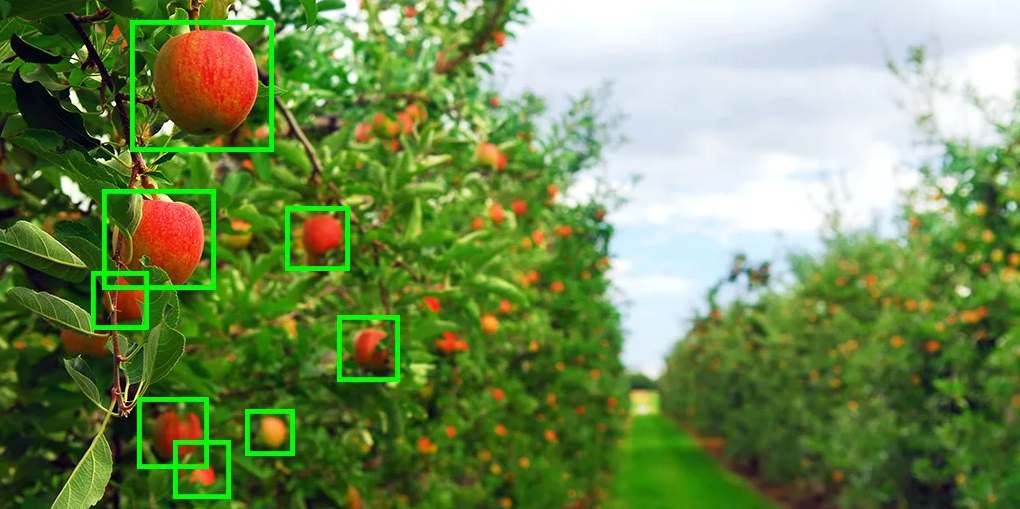
\includegraphics[width=0.8\textwidth]{figures/cv1.png} 
    \caption{Computer vision model applying object detection bounding boxes to identify apples within an orchard canopy..}
    \label{fig:computer_vision_matrix}
\end{figure}


In the state of the art robotic perception, deep neural models, capable of carrying out at the same time localization and classification, are built. These models are divided into two types of structures.

\begin{enumerate}
    \item \textbf{Two-Stage Detectors (e.g., Faster R-CNN):} To detect candidate regions before running classification and bounding-box regression, employ an RPN. These have high localization accuracy, though are computationally intensive.
    \item \textbf{One-Stage Detectors (e.g., YOLO series, SSD):} Structuralize object detection as a joint regression problem which maps pixel location to bounding box coordinates and class probabilities in one forward pass \cite{redmon2016you}. This makes their execution latency lower, which is good for mobile ground platforms.
\end{enumerate}

\subsubsection{Real-Time Decision Support}

The output of the deep learning network is directly passed to the robot's physical actuation layer. With high-confidence bounding boxes, Cartesian coordinates, and semantic pixel masks computed at high frame rates, the vision pipeline gives the navigation and spraying controllers with instantaneous position updates and hence allows immediate re-planning and precise local chemical applications.


\begin{itemize}
    \item \textbf{Local Processing:} These highly optimized deep neural networks are then implemented directly onto a local, low-power heterogeneous computing system (like the NVIDIA Jetson system), within the agriculture vehicle itself. All mathematical inference is done on-board.
    
    \item \textbf{Reduced Latency:} There is a very tight temporal requirement between classifying a target and initiating the actual nozzle actuation in agricultural robotics. The time requirement varies with forward velocity and is generally on the order of milliseconds. Edge computing removes transmission latency and data congestion from cloud communications, which is important for reliable operation in rural environments.
    \item \textbf{Real-Time Operation in the Field:} The onboard inference allows deterministic timings throughout the perception-actuation cycle. This synchronized latency allows the smart spraying platform to activate solenoid valves with normal operating times, thereby enabling precise application of chemicals to target weeds with no chance of slow actuation or undue chemical drift.
\end{itemize}
    







\section{Agricultural Challenges and Pesticide Application}

There are increased demands placed on agriculture to not only meet increasing global food demands but also to ensure agricultural practices are sustainable and economical. The FAO predicts substantial growth in food production will be required to feed the increasing global population which in turn demands more productive and efficient agricultural practices \cite{FAO2017}. In an attempt to do this pesticides are used extensively on our crops to combat pests and diseases which has effects on our yields and the quality of our food. Traditional spraying methods for pesticides, although widely used, are ineffective and pose risks to human health and the environment. Research states that a considerable percentage of the pesticides applied are wasted. This wastage, combined with its negative impacts to soil health, water systems and health risks to farmers, is one of the largest limitations of conventional pesticide applications \cite{Pimentel2005, Damalas2011}.


 \begin{figure}[H]
 \centering
 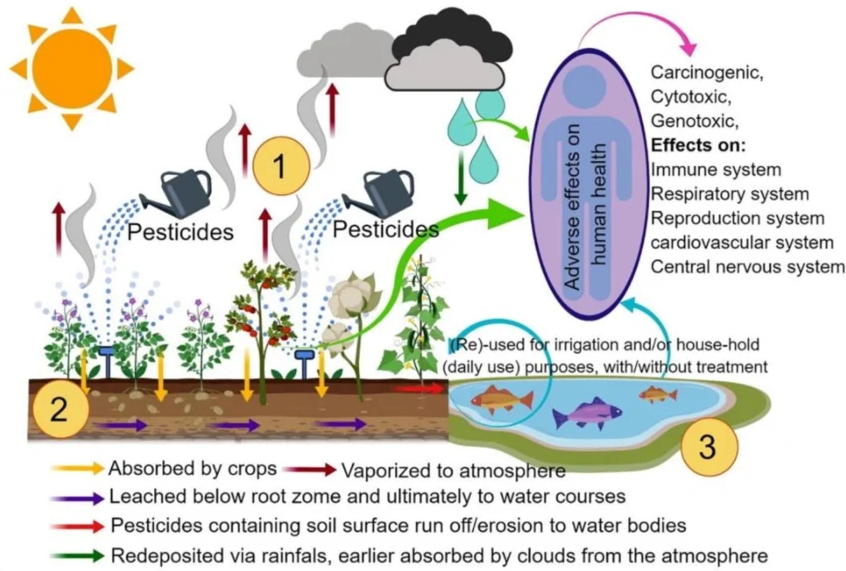
\includegraphics[width=0.8\linewidth]{figures/pesticide_impact.png}
 \caption{Environmental and health impacts of conventional pesticide application.}
 \label{fig:pesticide_impact}
 \end{figure}

\subsection{Growing Global Food Demand}
The growing world population, urbanization and altered eating habits are contributing to the increased food demand around the world. By 2050 the world population is anticipated to reach almost 10 billion; this needs considerable growth in agricultural production to attain food security \cite{FAO2017}. In conjunction with population growth, people in developed and developing countries due to rising income have started eating foods that requires more resources resulting in increased food demand. This puts great pressure on agricultural sector to fulfill the need of growing population by producing more food at a limited time span without compromising food quality and accessibility.

\begin{figure}[H]
    \centering
    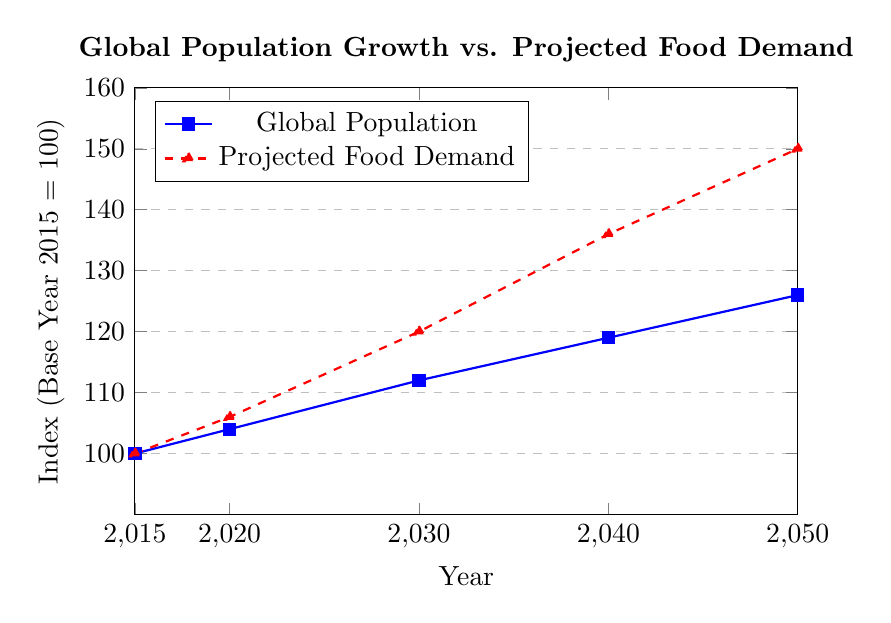
\begin{tikzpicture}
        \begin{axis}[
            title={\textbf{Global Population Growth vs. Projected Food Demand}},
            xlabel={Year},
            ylabel={Index (Base Year 2015 = 100)},
            xmin=2015, xmax=2050,
            ymin=90, ymax=160,
            xtick={2015, 2020, 2030, 2040, 2050},
            ytick={100, 110, 120, 130, 140, 150, 160},
            legend pos=north west,
            ymajorgrids=true,
            grid style=dashed,
            width=10cm,
            height=7cm
        ]
        
        % Line 1: Global Population Growth (Normalized index based on UN/FAO projections)
        \addplot[
            color=blue,
            mark=square*,
            thick
        ]
        coordinates {
            (2015, 100)
            (2020, 104)
            (2030, 112)
            (2040, 119)
            (2050, 126)
        };
        \addlegendentry{Global Population}
        
        % Line 2: Projected Food Demand (Typically outpaces population due to dietary shifts)
        \addplot[
            color=red,
            mark=triangle*,
            thick,
            dashed
        ]
        coordinates {
            (2015, 100)
            (2020, 106)
            (2030, 120)
            (2040, 136)
            (2050, 150)
        };
        \addlegendentry{Projected Food Demand}
        
        \end{axis}
    \end{tikzpicture}
    \caption{Projected trajectory of global population growth compared to total food demand up to 2050 (Adapted from FAO data). Food demand rises faster due to rising incomes and changing dietary preferences.}
    \label{fig:population_food_demand}
\end{figure}

\subsection{Pressure on Productivity and Sustainability}

The agricultural systems must enhance productivity while guaranteeing long term sustainability. Due to a limited extent for the increase of the agricultural lands-use, yield optimization becomes a fundamental challenge to be achieved. Simultaneously, the application of high intensive agricultural practices has induced environmental concerns such as land degradation, water scarcity and loss of bio-diversity. Sustainability means that the systems must reach high productivity and low environmental impact, aiming for resource use efficiency (water, fertilizers, pesticides etc.) \cite{Tilman2011}. The dual pressure necessitates the development of new technologies to attain the highest possible efficiency while ensuring no degradation to the environment.

\begin{table}[H]
    \centering
    \caption{Comparative Analysis of Conventional and Sustainable Agricultural Practices}
    \label{tab:conventional_vs_sustainable}
    \small 
    \setlength{\extrarowheight}{5pt} % Adds nice padding for multi-line text blocks
    
    % This custom column setup allocates space proportionally so the table doesn't look too wide
    \begin{tabularx}{\textwidth}{
        >{\hsize=0.4\hsize\linewidth=\hsize\raggedright\arraybackslash}X 
        >{\hsize=0.8\hsize\linewidth=\hsize\raggedright\arraybackslash}X 
        >{\hsize=0.8\hsize\linewidth=\hsize\raggedright\arraybackslash}X}
        \toprule
        
        \rowcolor[HTML]{2C3E50} % Dark slate header to match your other tables
        \textcolor{white}{\textbf{Aspect}} & 
        \textcolor{white}{\textbf{Conventional Approach}} & 
        \textcolor{white}{\textbf{Sustainable Approach}} \\
        \midrule
        
        \textbf{Pesticide Application} & 
        Blanket, calendar-based chemical spraying leading to high runoff and waste. & 
        Targeted, precision application using automated systems and integrated pest management (IPM). \\
        
        \rowcolor[HTML]{F2F4F4} % Light gray stripe
        \textbf{Environmental Impact} & 
        Severe soil degradation, chemical waste accumulation, and water contamination. & 
        Preservation of biodiversity, minimal chemical footprint, and soil health restoration. \\
        
        \textbf{Resource Efficiency} & 
        High input consumption (water, energy, chemicals) with significant volume loss. & 
        Resource-optimized application based on real-time crop needs and data tracking. \\
        
        \rowcolor[HTML]{F2F4F4} % Light gray stripe
        \textbf{Human Health Risk} & 
        Increased toxicity exposure for farmers, field workers, and nearby ecosystems. & 
        Controlled, minimized human contact and elimination of broad environmental drift. \\
        
        \textbf{Long-term Viability} & 
        Decreasing yields over time due to resistance and depleted soil quality. & 
        Resilient agricultural systems capable of meeting rising global food demands indefinitely. \\
        \bottomrule
    \end{tabularx}
\end{table}

\subsection{Constraints: Labor Shortages and Environmental Concerns}

Human input limitation is also apparent in agricultural productivity and increasing environmental regulation. The migration of population from rural to urban environments has resulted in limitations of labour, specifically for those repetitive, labour-intensive activities that are crucial to agriculture, such as spraying of pesticides \cite{Lowder2016}. This has been compounded by environmental fears, concerning chemicals such as soil contamination and water pollution, which are damaging to both agricultural practices and non-target organisms. Such constraints clearly suggest the necessity of alternatives, which minimize the necessity of manual labor yet are still efficient agricultural practice and environmentally prudent.
\begin{figure}[H]
    \centering
    % Adjust the width fraction (0.8) to make the image larger or smaller on your page
    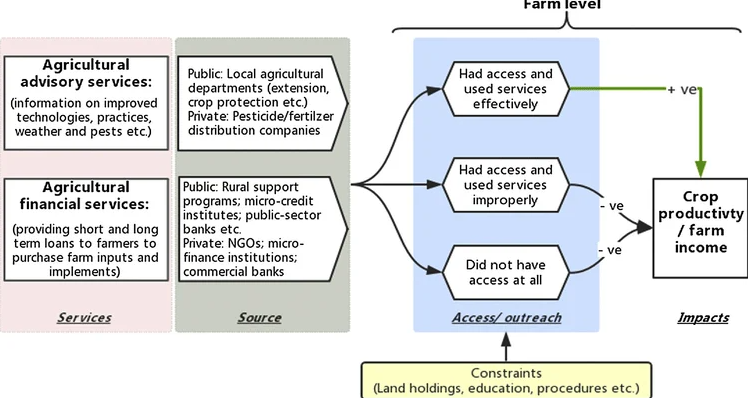
\includegraphics[width=0.8\textwidth]{figures/agricultural_constraints.png} 
    \caption{Conceptual framework of environmental and socioeconomic constraints acting on traditional agriculture, establishing the critical pathways that necessitate a transition toward smart automation.}
    \label{fig:agricultural_constraints}
\end{figure}


\subsection{Role and Limitations of Pesticide Use}

Modern agriculture relies heavily on the application of pesticides for weed, pest and disease control to assure high and stable crop yields and food quality. Globally pesticide use has lead to remarkable increases in food production and reduction in crop losses. However, despite their importance there are several issues with the current use of pesticides. Spray drift, evaporation and incorrect application lead to much of the pesticide never reaching its intended destination leading to a wasteful use of chemicals. This causes increase production costs and environmental pollution such as water contamination and harm to desirable organisms.

In addition to environmental considerations, pesticide exposure has severe health consequences to farmers and agricultural workers, especially in the developing world where there is often a lack of protective measures \cite{Damalas2011}. In these conditions, direct contact while mixing and spraying operations can cause both acute and chronic health effects. These risks are compounded by the practice of over-application, as farmers lack the accuracy to deliver an appropriate dosage using traditional methods. The failure to deliver accurate doses can have long-term consequences, in terms of both personal health and ecosystem damage, creating a case for improved, targeted methods of pesticide application.


\begin{figure}[H]
\centering
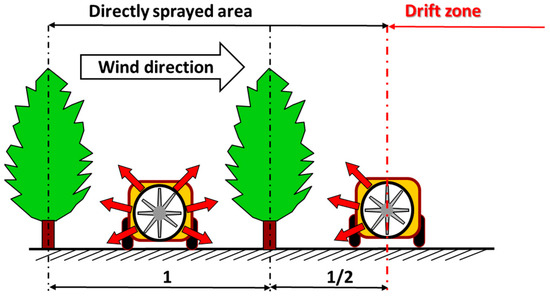
\includegraphics[width=0.8\linewidth]{figures/spray_drift.png}
 \caption{Illustration of pesticide spray drift and loss during conventional application.}
\label{fig:spray_drift}
 \end{figure}















 \section{Context and Motivation}

The work presented in this study builds upon a previous project focused on the development of an AI-based agricultural pest detection system. During the first phase, a computer vision model was developed and deployed on an roboflow platform, achieving an accuracy of approximately 85\% under the tested conditions. A simple pumping mechanism was also implemented to explore the feasibility of automated pesticide application.

However, the primary deliverable of the initial project was the detection model itself. While the results demonstrated promising detection performance, the model was not integrated into a complete robotic platform, and its practical suitability for real-world deployment remained largely unexplored. Furthermore, limited attention was given to software architecture, communication mechanisms, hardware-software integration, and system-level coordination.

To address these limitations, the present work focuses on the software engineering aspects required to support future agricultural robot development. Particular emphasis is placed on evaluating the deployment of the detection model within an embedded environment, establishing communication between system components, and designing software abstractions that facilitate interaction between hardware devices, processing units, and server-side services.

In addition, this work aims to provide a modular and maintainable software structure capable of supporting future prototypes and reducing the complexity of system integration. By addressing these architectural and communication challenges, the project contributes the foundational infrastructure necessary for the development and evaluation of more advanced intelligent agricultural systems.

% Suggested figure:
 \begin{figure}[h]
 \centering
 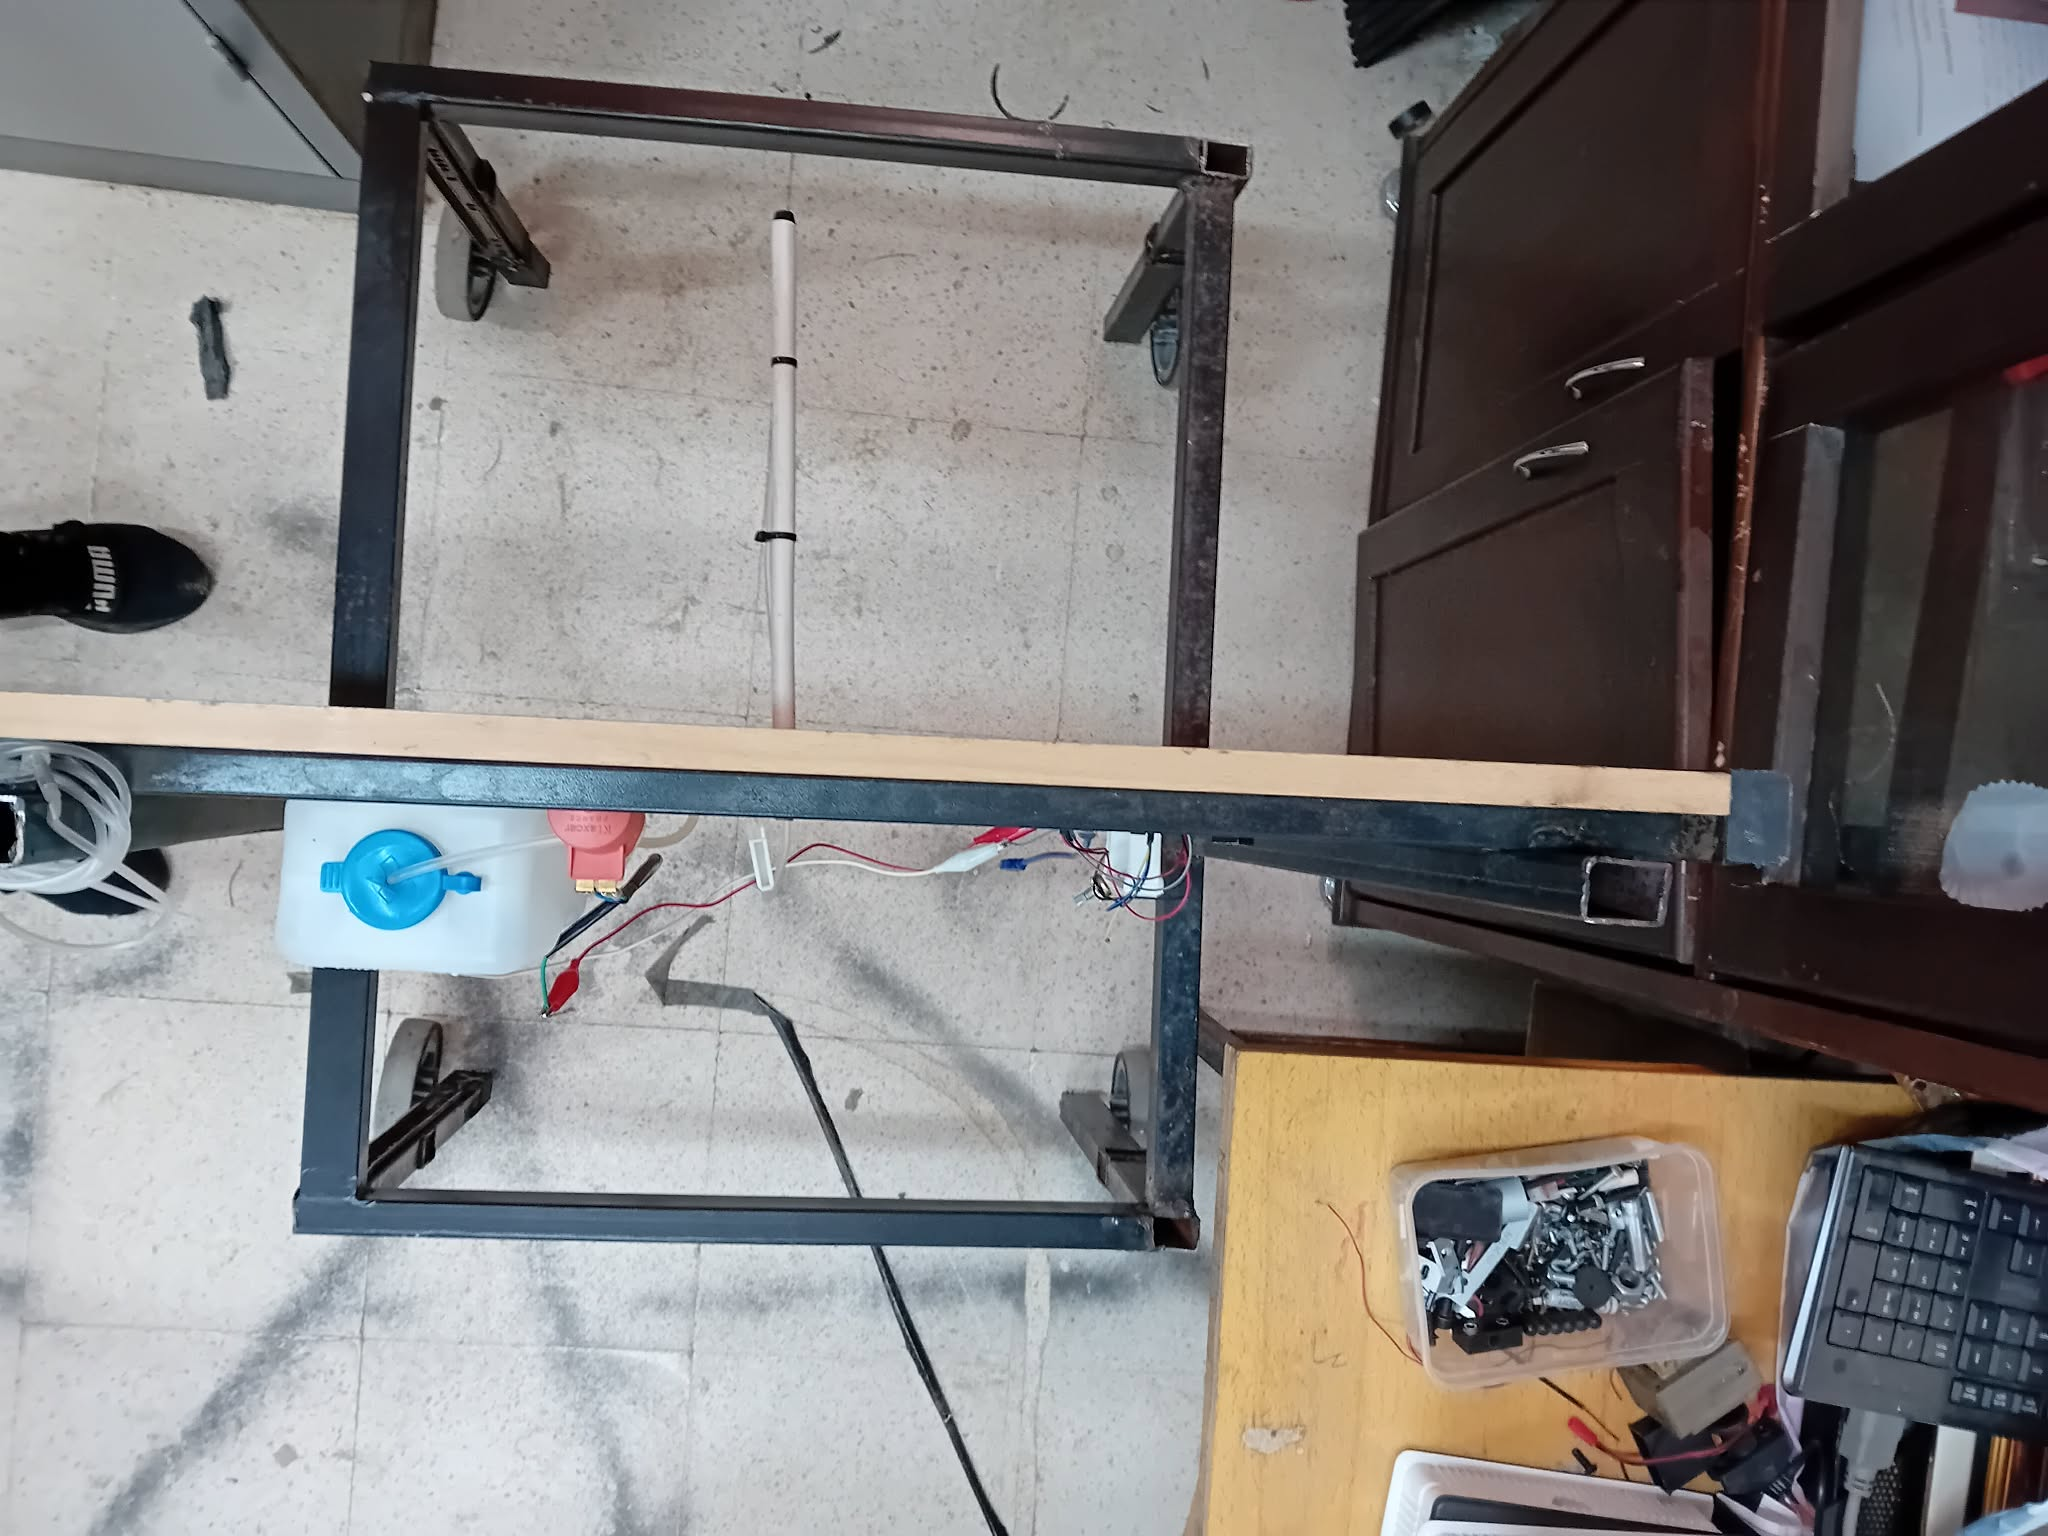
\includegraphics[width=0.8\linewidth]{figures/phase1_robot.png}
 \caption{Prototype developed in Phase 1.}
 \label{fig:phase1_robot}
 \end{figure}

\section{Problem Statement}

Although a pest detection model was successfully developed during the first phase of the project, its practical deployment within a complete agricultural robotic system remained unresolved. In particular, it was unclear whether the model could operate efficiently on embedded hardware and how it could be integrated with other system components in a reliable and maintainable manner.

The absence of a structured software architecture, standardized communication mechanisms, and clear component abstractions makes the development and integration of future prototypes unnecessarily complex. As a result, there is a need for a software framework that facilitates communication between embedded devices, AI processing modules, and server-side services while supporting the evaluation of AI model deployment in real-world conditions.

This work addresses the following research question:

\begin{quote}
\textbf{How can a robust software architecture be designed to support communication, integration, and deployment of AI-based agricultural systems while enabling the evaluation of model practicality on embedded platforms?}
\end{quote}


To answer this question we must address a series of sub-questions:


\begin{enumerate}
    \item What communication mechanisms can be used to enable reliable interaction between embedded devices, AI processing modules, and server-side services?
    
    \item What software abstractions and architectural patterns can improve the maintainability, extensibility, and integration of agricultural robotic systems?
    
    \item What challenges arise when deploying the existing pest detection model on embedded hardware platforms?
    
    \item To what extent is the previously developed detection model suitable for practical deployment within an integrated agricultural system?
    
    \item How can the proposed software architecture support future development and integration of additional system components?
    \item What system architecture enables seamless integration of computer vision, and spraying control?
    
    \item What safety, fault-tolerance, and redundancy mechanisms are required to ensure reliable operation?
\end{enumerate}

These are just some of the difficulties, indicating that the problem is cross-disciplinary, combining robotics, artificial intelligence, embedded systems and precision agriculture methods.


\section{Project Objectives}

The purpose of this project is to establish the software foundations required for the integration and evaluation of AI-based agricultural systems. Rather than focusing on the development of new detection algorithms, this work concentrates on software architecture, communication mechanisms, and embedded deployment challenges that must be addressed before a practical agricultural robot can be realized.

\subsection{Functional Objectives}

The functional objectives are as follows:
\begin{itemize}
    \item Integrate the existing pest detection model within a software framework suitable for embedded environments.
    \item Develop communication mechanisms that enable interaction between embedded devices, AI processing modules, and server-side services.
    \item Evaluate the feasibility and limitations of deploying the detection model on embedded hardware.
    \item Provide monitoring and management capabilities through a centralized software platform.
\end{itemize}

\subsection{Technical Objectives}

The technical objectives include:
\begin{itemize}
    \item Design a modular and extensible software architecture that supports future system development and integration.
    \item Define software abstractions that simplify communication and coordination between system components.
    \item Improve the maintainability, scalability, and reliability of the overall system structure.
    \item Establish a software foundation that facilitates the development of future agricultural robot prototypes.
\end{itemize}

\noindent These objectives aim to bridge the gap between a standalone AI detection model and a more integrated agricultural system while providing a framework that can support future research and development efforts.
